\documentclass[11pt]{article}
%基于北京航空航天大学仪器科学与光电工程学院实验报告及课程报告排版得来,类似于毕业论文排版格式
%后续将更新毕业论文排版格式
\usepackage{graphicx,float}%使用图的宏包,使用图的浮动体宏包,引入参数H使图像紧跟当前文字
\usepackage{caption} %使用图表标题的宏包
\usepackage[colorlinks=true,pdfstartview=FitH,%
linkcolor=black,anchorcolor=violet,citecolor=magenta]{hyperref}%加载hyperref宏包,使用超链接
\usepackage{setspace}%用于设置行间距列间距等命令的宏包
\usepackage{array}%设置列表高度宽度的宏包
\usepackage{zhnumber}%使用中文数字编号的宏包
\usepackage{titlesec,titletoc}%使用标题自定义形式的宏包和使用目录自定义形式的宏包
\usepackage{siunitx}%物理学单位宏包
\usepackage{tabularx}%让表格宽度等于页面宽度
\usepackage{makecell}%单个表格单元调整的宏包
\usepackage{subfigure} %%使用子图的宏包
\usepackage[backend=biber,bibstyle=gb7714-1987,%nature,%%加载biblatex宏包,使用参考文献
citestyle=gb7714-1987%,backref=true%%其中后端backend使用biber
,url=false
]{biblatex}%标注(引用)样式citestyle,著录样式bibstyle都采用gb7714-2015样式
% \usepackage{pgfplots}%类似tikz的一个画图库,主要画统计图
\usepackage{../customStyle}
% \usepackage{customFont}%自行编写的字体命令库,基于CJK宏包
% \usepackage{bh_style}%自行编写的风格文件,基于使用习惯和格式要求
% \usepackage{math_formulate}%自行编写的数学公式命令库,基于amsmath宏包
% \usepackage{picture}%集成图形绘制库,主要包括了tikz和pgfplots两大主流宏包
% \usepackage[lite,subscriptcorrection,slantedGreek,nofontinfo]{mtpro2}%使用mathtimepro2商业字体作为数学环境,并不推荐

%biblatex宏包的参考文献数据源加载方式,注意book.bib应当与.tex文件在同一目录下,不然有可能会报错
\addbibresource[location=local]{book.bib}
% % \bibliographystyle{gbt7714-numerical}
%%% 下面的命令重定义页面边距,使其符合中文刊物习惯 %%%%
% \addtolength{\topmargin}{2.5cm}
\setlength{\oddsidemargin}{0.63cm}  % 3.17cm - 1 inch
\setlength{\evensidemargin}{\oddsidemargin}
% \setlength{\textwidth}{14.66cm}
% \setlength{\textheight}{24.00cm}    % 24.62

\graphicspath{{./fig}}

\begin{document}
{
\pagestyle{empty}
\begin{figure}
  
\includegraphics{title.jpg}
\end{figure}
\begin{center}

  \begin{figure}[h]

    \centering
    
\includegraphics[]{title.png}\par
    \vspace{4em}
    \large{\yihao\lishu{2023-2024学年第一学期}}
    \vspace{6em}
  \end{figure}

  \large{\erhao\lishu{随机过程理论}}\par
  \large{\erhao\lishu{课程大作业合集}}
  \vspace{8em}

  \begin{spacing}{2.0}
    \begin{tabular}{cc}


      {\xiaoerhao\lishu{班\quad \quad 级}} & {\heiti{\dlmu{SY23173}}}    \\
      {\xiaoerhao\lishu{学\quad \quad 号}} & {\heiti{\dlmu{SY2317301} }} \\
      {\xiaoerhao\lishu{姓\quad \quad 名}} & {\heiti{\dlmu{陈博非} }}       \\
      {\xiaoerhao\lishu{日\quad \quad 期}} & {\heiti{\dlmu{\today} } }   \\
    \end{tabular}
  \end{spacing}
\end{center}
\thispagestyle{empty}
}


\newpage
%手动分页
\pagenumbering{roman}

\setcounter{tocdepth}{3}
%设定目录深度                      
\tableofcontents
%列出目录
\newpage

\pagenumbering{arabic}
\setcounter{page}{1}
\section{第一次大作业}
\subsection{问题描述}
为了生成两个完全不相关的随机信号,现如下图设计了一个信号滤波器,其中输入为一随机信号,两个输出为需要的不相关随机信号。
\begin{figure}[H]
  \centering
  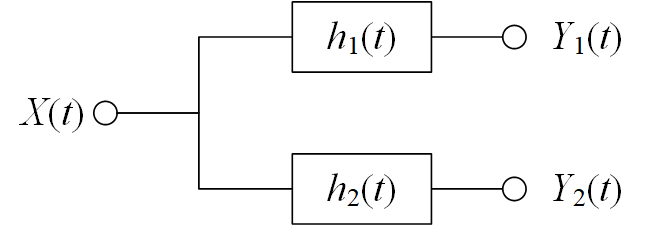
\includegraphics[width=0.8\textwidth]{信号发生器示意图.png}
  \caption{信号滤波器}
  \label{fig:信号滤波器}
\end{figure}

\subsection{设计思路}
首先从原理上讨论应该如何设计两个线性系统,考虑两个输出信号之间的互相关函数。即有:
\begin{equation}
  \begin{aligned}
    R_{XY}(t_1,t_2) & =E\{y_1(t_1)y_2(t_2)\}                                                                                               \\
                    & =E\{[x_1(t)*h_1(t)][x_2(t)*h_2(t)]\}                                                                                 \\
                    & =E\Big\{\int_{-\infty}^{+\infty}x_1(u)h_1(t_1-u)\mathrm{d}u\int_{-\infty}^{+\infty}x_2(v)h_2(t_2-v)\mathrm{d}v\Big\} \\
                    & =\int_{-\infty}^{+\infty}\int_{-\infty}^{+\infty}h_1(t_1-u)h_2(t_2-v)E[x_1(u)x_2(v)]\mathrm{d}u\mathrm{d}v           \\
                    & =\int_{-\infty}^{+\infty}\int_{-\infty}^{+\infty}R_x(u,v)h_1(t_1-u)h_2(t_2-v)\mathrm{d}u\mathrm{d}v                  \\
                    & =R_x(t_1,t_2)*h_1(t_1)*h_2(t_2)
  \end{aligned}
\end{equation}
可见,两个输出信号之间的互相关函数相当于对输入信号的自相关函数进行两次卷积,如果输入的函数是平稳的,两个输出的信号之间是联合平稳的,则可以使用功率谱密度函数表示上述结果,得到以下形式:
\begin{equation}
  \begin{aligned}
    S_{XY}(\omega) & =S_X(\omega)H_1(\omega)H_2^*(\omega)
  \end{aligned}
\end{equation}
可见,当两个输出信号之间的互相关函数为零时,功率谱密度函数也为0,则需要两个线性系统的频率响应函数在每一个频率上均是乘积为0的。换言之,需要设计两个线性系统,使得两个系统的频率响应函数不为零的位置相互错开,即可得到两个输出不相关的信号。

考虑最简单的情况,即设计一个低通滤波器和一个高通滤波器,使得两个滤波器的截止频率相互错开,其在频率上的乘积即可以满足近似为0。工程上,认为阻带内的衰减小于-15dB即可认为是0,滤波器的截止频率定义为幅频增益为-3dB处的频率。\cite{signal_system}。
\subsection{设计过程}
由于问题没有给任何信号的具体形式,这里也没有必要定义某一个具体的截止频率,不妨设低通滤波器的截止频率(角频率)是$\omega_1$,高通滤波器的截止频率是$\omega_2$,则有:
\subsubsection{低通滤波器}
如下图,低通滤波器的幅频特性为:
\begin{figure}[H]
  \centering
  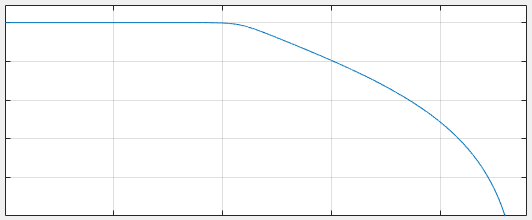
\includegraphics[width=0.8\textwidth]{低通滤波器.png}
  \caption{低通滤波器幅频特性说明}
  \label{fig:低通滤波器}
\end{figure}

可将低通滤波器的频率特性写为:
\begin{displaymath}
  H_1(j\omega)=\frac{1}{\displaystyle 1+j\frac{\omega}{\omega_L}}
\end{displaymath}
其中$\omega_L$为截止频率。
\subsection{高通滤波器}
同理,对于高通滤波器,其幅频特性为:
\begin{figure}[H]
  \centering
  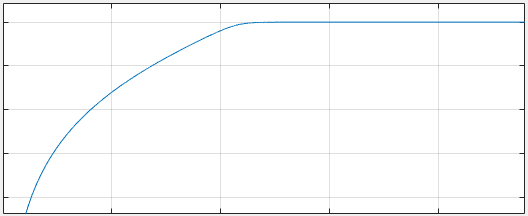
\includegraphics[width=0.8\textwidth]{高通滤波器.png}
  \caption{高通滤波器幅频特性说明}
  \label{fig:高通滤波器}
\end{figure}
可将高通滤波器的频率特性写为:
\begin{displaymath}
  H_2(j\omega)=\frac{1}{\displaystyle 1+j\frac{\omega_H}{\omega}}
\end{displaymath}
其中$\omega_H$为高通截止频率。
\subsubsection{设计结果}
需要注意的是,首先应当保证高通滤波器的截止频率高于低通滤波器的截止频率,即有:
\begin{equation*}
  \omega_2>\omega_1
\end{equation*}

其次是为了保证在任意频率处的幅值增益都小于-15dB,则需要在两个幅频特性相等的位置处,幅值增益的和也小于-15dB,即有:
\begin{align}
  \left\{
  \begin{aligned}
     & 20\lg\mmode{\frac{1}{\displaystyle 1+j\frac{\omega}{\omega_L}}}=20\lg\mmode{\frac{1}{\displaystyle 1+j\frac{\omega_H}{\omega}}}     \\\\
     & 20\lg\mmode{\frac{1}{\displaystyle 1+j\frac{\omega}{\omega_L}}}+20\lg\mmode{\frac{1}{\displaystyle 1+j\frac{\omega_H}{\omega}}}<-15
  \end{aligned}
  \right.
\end{align}
对于某一个给定的截止频率,可得两幅频特性曲线之交点频率,以及两个截止频率需要满足的条件为:
\begin{align*}
  \left\{
  \begin{aligned}
     & \omega=\sqrt{\omega_H\omega_L}                       \\\\
     & \frac{\omega_L^2}{\omega_H^2+\omega_L^2}<10^{-0.375}
  \end{aligned}
  \right.
\end{align*}
因此可以设计得到在任意频率点处,均可以以-15dB负增益。则从输入到输出的功率谱密度函数为:
\begin{align*}
  S_{XY}(\omega)=\frac{S_X(\omega)}{\displaystyle 1+\frac{\omega_H}{\omega_L}+j\circbrac{-\frac{\omega_H}{\omega}+\frac{\omega}{\omega_L}}}
\end{align*}
其中,一个比较简单的实现形式为:
\begin{align*}
  H_1(j\omega)=\frac{1}{\displaystyle 1+j\frac{\omega}{\omega_L}} \implies h_1(t)=\left\{
  \begin{aligned}
     & e^{\displaystyle -\frac{1}{\omega_L}t} & ,  t>0   \\
     & 0                                      & ,  t\le0
  \end{aligned}
  \right.
\end{align*}

\begin{align*}
  H_2(j\omega)=\frac{1}{\displaystyle 1+j\frac{\omega_H}{\omega}} \implies h_1(t)=\left\{
  \begin{aligned}
     & 0                                               & , t>0   \\
     & \delta(t)-e^{\displaystyle \frac{1}{\omega_H}t} & , t\le0
  \end{aligned}
  \right.
\end{align*}\par
这里的高通滤波器是物理不可实现的,因此常常使用巴特沃斯滤波器或者切比雪夫滤波器形式的函数实现高通滤波,而不是使用指数函数的形式,给定截止频率和阻带衰减,即可以设计出对应的高通滤波器。
\section{第二次大作业}
\subsection{概述}
%分析一个应用泊松随机过程的实例。
本文将主要讨论一种新型的神经网络模型,即脉冲神经网络(Spiking Neural Networks,SNN)。该网络据传是继感知机、卷积神经网络之后所谓的第三代类脑仿生网络模型,与前两代神经网络相比,脉冲神经网络在能耗上和存储占用上有着更加突出的优点。但是,当前脉冲神经网络的研究还很不充分,尚未形成一种通用的数学模型基础,因此其模型底层原理、模型训练方法以及模型的推理方法均未见到有通行的方法,大多数研究尚局限在某一具体方法中的应用。从大脑工作机理的仿生学中抽象数学模型、完成对神经元和网络连接拓扑的建模,是当前脉冲神经网络原理领域需要深入研究的工作。本文将针对这一问题,利用随机过程数学工具,对脉冲神经元进行建模,以期望能够归纳出一种通行的模型范式。
\subsection{符号说明}
SNN的输入与输出均是脉冲型信号,根据文献\cite{jaegerEncyclopediaComputationalNeuroscience2015},首先给出以下符号表示。
\begin{enumerate}
  \item 脉冲\textbf{电流信号}使用增量序列表示,记为$X(t)$,常用冲激函数串表示:$X(t)=\sum\limits_i\delta(t-t_i)$,其中$t_i$是产生事件的时刻。神经元的输入电流记为$X_i(t)$,输出电流记为$Y(t)$;
  \item 神经元膜内外电位差用符号$V(t)$表示,简称为“膜电位”;
  \item 神经元放电的阈值膜电位记为$V_T$;
  \item 神经元膜电位时间常数为$\tau$,膜电阻记为$r$;
\end{enumerate}
\subsection{脉冲神经元模型}
脉冲神经元是对神经元细胞生物机理的仿生抽象。根据神经细胞领域的研究\cite{albesa-gonzalezLearningFilopodiaSpines2023},神经元仅当其动作电位(Active Potential)高于其活动阈值后,神经元细胞膜表面的离子通道(通常是钾、钙离子通道)在膜内外电位差的驱动下打开,神经元膜内的钾离子和钙离子将在极短的时间内从膜内释放至膜外,宏观上形成了一次放电时间极短的输出电流,在数学上通常建模为一次总放电能量有限但功率无限的信号,即冲激信号。\par
神经元彼此间通过突触连接,突触是一种化学物质受体,用于接受前一个神经元释放的神经介质。例如,当前一个神经元兴奋时(即产生正电流输出),其释放的神经介质通常为谷氨酸(Glutamate),谷氨酸将与突触上的受体结合,使得后一个神经元膜上的抽运离子通道打开,后一个神经元膜内钠离子浓度提高,导致其膜电位升高。而当前一个神经元抑制时(即产生负电流输出),其释放的神经介质通常为$\gamma$-氨基丁酸(GABA),GABA将与突触上的受体结合,导致后一个神经元抽运阴离子至胞内(常为氯离子),使其膜电位下降。根据离子扩散现象,胞内的高浓度离子也将自发地穿过细胞膜扩散至膜外直到膜两则浓度相同,当神经元长期处于静息状态时,其离子扩散速率等于神经元的抽运速率,膜电位基本稳定在某一固定值。\par
常用的模型是漏积分放电(Leaky Integrate-and-Fire,LIF)神经元\cite{gerstnerTimeStructureActivity1995},即神经元将全部输入脉冲进行时间延迟的线性叠加,其与膜时间常数有关,微分方程为:
\begin{align}
  \tau\diff{V(t)}{t}=-V(t)+r\sum\limits_iX_i(t)
  \label{eq:LIF积分过程}
\end{align}\par
式中,$X_i(t)$是第$i$个输入脉冲电流,如神经元有多个输入,则将其线性叠加;$-V(t)$描述了离子扩散速率,当膜电位较大时,扩散速度较大,因此符合前述一般性假设。神经元的行为不止有积分过程,当膜电位超过膜电位阈值时,神经元放电过程将被激活(Fire),放电过程不是线性过程,可用分段函数表示为:
\begin{align}
  Y(t)=\begin{cases}
         1 & ,V(t)>V_T    \\
         0 & ,V(t)\le V_T
       \end{cases}\implise Y(t)=u(V(t)-V_T)
  \label{eq:LIF放电过程}
\end{align}

\newpage
\printbibliography[heading=bibliography,title=参考文献]
\end{document}
